%%%%%%%%%%%%%%%%%%%%%%%%%%%%%%%%%%%%%%%%%
% Short Sectioned Assignment
% LaTeX Template
% Version 1.0 (5/5/12)
%
% This template has been downloaded from:
% http://www.LaTeXTemplates.com
%
% Original author:
% Frits Wenneker (http://www.howtotex.com)
%
% License:
% CC BY-NC-SA 3.0 (http://creativecommons.org/licenses/by-nc-sa/3.0/)
%
%%%%%%%%%%%%%%%%%%%%%%%%%%%%%%%%%%%%%%%%%

%----------------------------------------------------------------------------------------
%	PACKAGES AND OTHER DOCUMENT CONFIGURATIONS
%----------------------------------------------------------------------------------------

\documentclass[paper=a4, fontsize=11pt]{scrartcl} % A4 paper and 11pt font size

\usepackage[T1]{fontenc} % Use 8-bit encoding that has 256 glyphs
%\usepackage{fourier} % Use the Adobe Utopia font for the document - comment this line to return to the LaTeX default
\usepackage[english]{babel} % English language/hyphenation
\usepackage{amsmath,amsfonts,amsthm} % Math packages
\usepackage{mathtools} %More math! (For dscases)
\usepackage{hyperref} %HTML package
\usepackage{pgfplots} %Makes plots in LaTeX
\usepackage{tikz} %Also tikz?
\usepackage{bm} %makes vectors bold
\usepackage{bbm} %Blackboard bold 1
\usepgfplotslibrary{fillbetween}%Let's me fill between named plots
\usepackage{graphicx} %import pics
\graphicspath{ {Python_figs/} }
\DeclareGraphicsExtensions{.pdf,.png,.jpg}
\usepackage{sectsty} % Allows customizing section commands
\allsectionsfont{ \normalfont\scshape} % Make all sections the default font and small caps


\renewcommand{\thesubsection}{\alph{subsection}} %Make subsections start with letters

\usepackage{fancyhdr} % Custom headers and footers
\pagestyle{fancyplain} % Makes all pages in the document conform to the custom headers and footers
\fancyhead{} % No page header - if you want one, create it in the same way as the footers below
\fancyfoot[L]{} % Empty left footer
\fancyfoot[C]{} % Empty center footer
\fancyfoot[R]{\thepage} % Page numbering for right footer
\renewcommand{\headrulewidth}{0pt} % Remove header underlines
\renewcommand{\footrulewidth}{0pt} % Remove footer underlines
\setlength{\headheight}{13.6pt} % Customize the height of the header

\numberwithin{equation}{section} % Number equations within sections (i.e. 1.1, 1.2, 2.1, 2.2 instead of 1, 2, 3, 4)
\numberwithin{figure}{section} % Number figures within sections (i.e. 1.1, 1.2, 2.1, 2.2 instead of 1, 2, 3, 4)
\numberwithin{table}{section} % Number tables within sections (i.e. 1.1, 1.2, 2.1, 2.2 instead of 1, 2, 3, 4)

\setlength\parindent{0pt} % Removes all indentation from paragraphs - comment this line for an assignment with lots of text

\usepackage{listings}
\lstset{language=Python}


%----------------------------------------------------------------------------------------
%	TITLE SECTION
%----------------------------------------------------------------------------------------

\newcommand{\horrule}[1]{\rule{\linewidth}{#1}} % Create horizontal rule command with 1 argument of height

\title{	Assignment 2}

\author{Benjamin Jakubowski} % Your name

\date{\normalsize\today} % Today's date or a custom date

\begin{document}

\maketitle % Print the title

%----------------------------------------------------------------------------------------
%	PROBLEM 1.1
%----------------------------------------------------------------------------------------

\section*{1. Preliminaries}
\subsection*{1.1 Dataset construction}

See attached iPython notebook.

%----------------------------------------------------------------------------------------
%	PROBLEM 1.2
%----------------------------------------------------------------------------------------

\subsection*{1.2 Experiments with Ridge Regression}

Ridge regression was run on the simulated dataset for a range of $\lambda$ values, and performance was evaluated using validation set square loss. The optimal $\lambda_{opt}$ (i.e. validation set square loss minimizing $\lambda$) was found to be $1.6 \times 10^{-5}$. A plot showing results (near $\lambda_{opt}$) is shown below:
\begin{center} 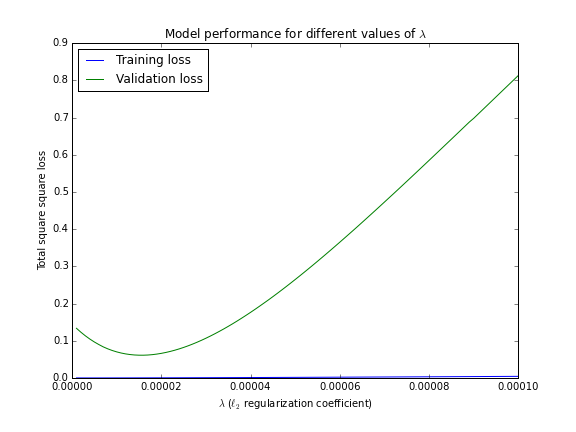
\includegraphics[scale=0.65]{./../figures/1_2_1.png} \end{center}

Next, let's examine the minimizing weight vector $\bm{w}$ found when $\lambda = 1.6 \times 10^{-5}$; specifically, we're interested in the number of coefficients $w_j$ at or near zero. These results are presented in the table below:

\begin{itemize}
\item $w_j = 0$:

\begin{center}
\begin{tabular}{| c | c | c |}
\hline
	& Predicted zero &  Predicted non-zero\\
\hline
True non-zero ($\bm{w}$[0:10]) &  0 &  10 \\
\hline
True zero ($\bm{w}$[10:]) & 0 & 65 \\
\hline
\end{tabular}\end{center}

\item $w_j < 10^{-3}$:

\begin{center}
\begin{tabular}{| c | c | c |}
\hline
	& Predicted zero &  Predicted non-zero\\
\hline
True non-zero ($\bm{w}$[0:10]) &  0 &  10 \\
\hline
True zero ($\bm{w}$[10:]) & 0 & 65 \\
\hline
\end{tabular}\end{center}

\item $w_j < 10^{-2}$:

\begin{center}
\begin{tabular}{| c | c | c |}
\hline
	& Predicted zero &  Predicted non-zero\\
\hline
True non-zero ($\bm{w}$[0:10]) &  0 &  10 \\
\hline
True zero ($\bm{w}$[10:]) & 5 & 60 \\
\hline
\end{tabular}\end{center}

\item $w_j < 10^{-1}$:

\begin{center}
\begin{tabular}{| c | c | c |}
\hline
	& Predicted zero &  Predicted non-zero\\
\hline
True non-zero ($\bm{w}$[0:10]) &  0 &  10 \\
\hline
True zero ($\bm{w}$[10:]) & 37 & 28 \\
\hline
\end{tabular}\end{center}

\end{itemize}

It is apparent that ridge regression is achieving shrinkage, but not promoting sparsity (i.e. setting coefficients to 0).

%----------------------------------------------------------------------------------------
%	PROBLEM 2.1
%----------------------------------------------------------------------------------------

\section*{2. Coordinate Descent for Lasso (Shooting Algorithm)}
\subsection*{2.1 Experiments with the Shooting Algorithm}
\subsubsection*{2.1.1 Finding an optimal $\lambda$}

First, the (non-vectorized, i.e. looping) lasso coordinate descent algorithm was implemented (see attached iPython notebook). Using this implementation, the optimal (i.e. validation set square error minimizing) $\lambda$ was found to be ~0.596, with a corresponding validation set square error of $7.51 \times 10^{-3}$. Loss values for $\lambda$ in a neighborhood of $\lambda_{opt} = 0.596$ are shown in the plot below:

\begin{center} 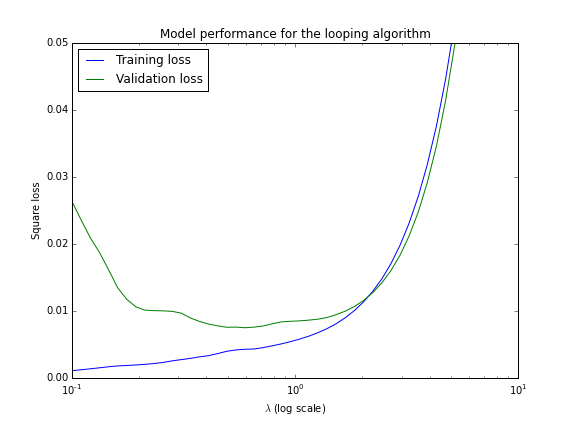
\includegraphics[scale=0.65]{./../figures/2_1_looping.png} \end{center}

\subsubsection*{2.1.2 Sparsity analysis of $\bm{w_{\lambda_{opt}}}$}

First, prior to analyzing the sparsity of our solution, we present a learning curve showing the number of zero coefficients versus the number of iterations of the cyclic coordinate descent algorithm.\\
\begin{center} 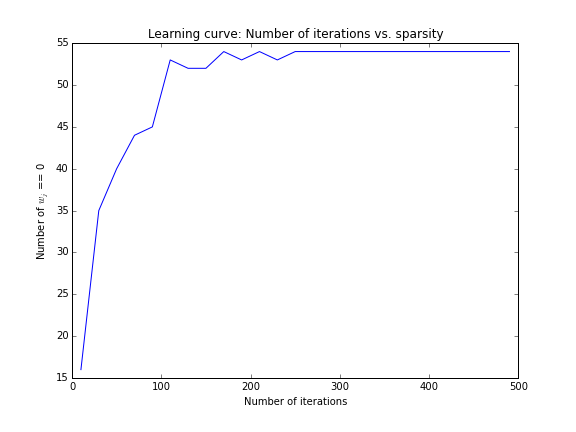
\includegraphics[scale=0.65]{./../figures/2_1_2.png} \end{center}

Based on this learning curve, it appears the sparsity of our solution stabilizes when the number of iterations is greater than 250. Thus, setting the number of iterations to 300, we report a "confusion matrix" for the zero/non-zero coefficients of $\bm{w}$.

\begin{center}
\begin{tabular}{| c | c | c |}
\hline
	& Predicted zero &  Predicted non-zero\\
\hline
True non-zero ($\bm{w}$[0:10]) &  0 &  10 \\
\hline
True zero ($\bm{w}$[10:]) & 54 & 11 \\
\hline
\end{tabular}\end{center}
Importantly, the maximum absolute value of the 15 predicted non-zero, true zero coefficients was $0.0548$. Thus, compared to the true non-zero weights (which ranged in absolute value between 9.9 and 10.04), the lasso essentially assigned no weight to the true zero features.

\subsubsection*{2.1.3 Implementing the homotopy method}

The homotopy method was implemented as follows:
\begin{itemize}
\item The same candidate set for $\lambda$ was chosen as in 2.1.1 (specifically the set defined by \texttt{np.logspace(-1,1, 50)}).
\item The homotopy algorithm was initialized with the same starting weight vector as the looping algorithm (namely the optimal $\bm{w}$ found using ridge regression), and with $\lambda = \max$(\texttt{np.logspace(-1,1, 50)}).
\item For each $\lambda \in $ \texttt{np.logspace(-1,1, 50)}, the optimal weight vector found in the previous iteration was used as the starting point for the coordinate descent.
\end{itemize}

Results from the homotopy method (used with the looping algorithm) are presented below

\begin{center} 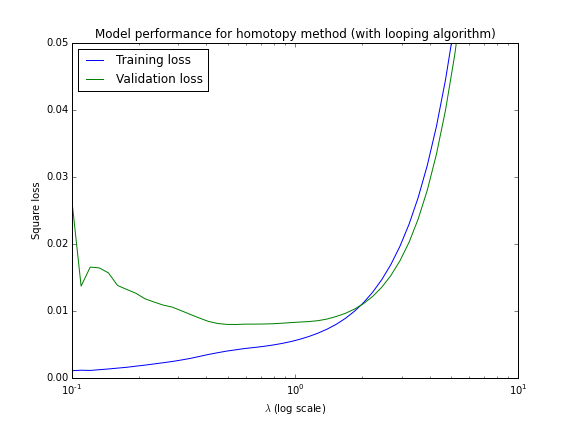
\includegraphics[scale=0.65]{./../figures/2_1_3.png} \end{center}

Next, runtimes for the two algorithms were compared:

\begin{center}
\begin{tabular}{| c | c |}
\hline
	\textbf{Implementation (tolerance $= 10^{-6}$) } & \textbf{Runtime}\\
\hline
	Looping with homotopy method & \texttt{1 loops, best of 3: 4min 5s per loop} \\
\hline
	Looping without homotopy method &  \texttt{1 loops, best of 3: 4min 17s per loop} \\
\hline
\end{tabular}
\end{center}

Thus, it appears the homotopy method achieved marginal runtime gains. Note this result might be due to the termination conditions used for both algorithms. Both algorithms terminated after either:
\begin{itemize}
\item 100 iterations (cycles through each coordinate)
\item $\bm{w_{i+1}}$ - $\bm{w_{i}}$ < tolerance $= 10^{-6}$
\end{itemize}
Perhaps the tolerance was too strict, so termination was essentially determined by the fixed maximum number of iterations- if so, the homotopy wouldn't produce any runtime gains.

To test this hypothesis, the test was re-run with tolerance $=  10^{-3}$. Runtime results from this test are given below:

\begin{center}
\begin{tabular}{| c | c |}
\hline
	\textbf{Implementation (tolerance $= 10^{-3}) $ } & \textbf{Runtime}\\
\hline
	Looping with homotopy method & \texttt{1 loops, best of 3: 4min 44s per loop} \\
\hline
	Looping without homotopy method &  \texttt{1 loops, best of 3: 1min 16s per loop} \\
\hline
\end{tabular}
\end{center}

Thus, with the tolerance set to a lower value ($10^{-3}$), we see the homotopy method producing a substantial runtime improvement.

\subsubsection*{2.1.4 Vectorizing the coordinate descent algorithm}

First we present matrix expressions for computing $a_j$ and $c_j$ in the coordinate descent algorithm. Recall
\begin{align*}
a_j &= 2 \sum_{i=1}^n x_{ij}^2 \\
c_j &= 2  \sum_{i=1}^n x_{ij} (y_i - w^T x_i + w_jx_{ij})
\end{align*}
Then, first letting
\begin{itemize}
\item ${X_{.j}}$ be the $j^{th}$ column (i.e. feature) of matrix $X$
\item $X_{.-j}$ be the matrix $X$ without the $j^{th}$ column (feature)
\item $w_{-j}$ be the weight vector $w$ without the $j^{th}$ entry
\end{itemize}
we can expressed $a_j$ and $c_j$ in matrix/vector notation as:
\begin{align*}
a_j &= 2 X_{.j}^T X_{.j} \\
c_j &= 2 X_{.j}^T\ (y - X_{.-j} w_{-j})
\end{align*}

After implementing the vectorized algorithm, the following results were obtained:

\begin{center} 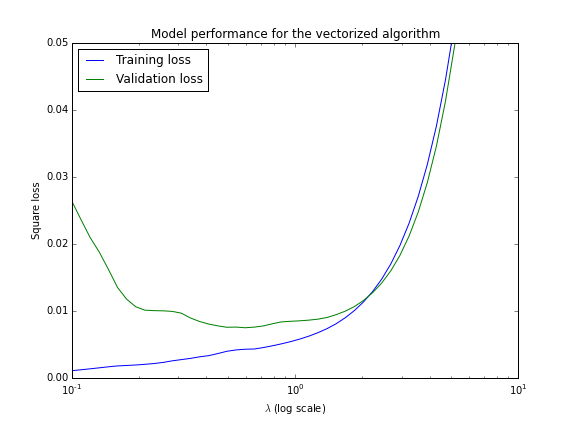
\includegraphics[scale=0.65]{./../figures/2_1_vectorized.png} \end{center}

First, it is important to note the model performance (i.e. square loss for a given $\lambda$) is equivalent under the looping and the vectorized versions of the looping algorithm. However, the runtimes are very different. Using $\texttt{\%timeit}$ magic in iPython for $\lambda = 0.596$, with a maximum of 100 iterations and tolerance = $10^{-6}$, and initializing with the solution to the ridge regression problem, the following runtimes were obtained:

\begin{center}
\begin{tabular}{| c | c |}
\hline
	\textbf{Implementation} & \textbf{Runtime}\\
\hline
	Vectorized & \texttt{1 loops, best of 3: 332 ms per loop} \\
\hline
	Looping &  \texttt{1 loops, best of 3: 4.62 s per loop} \\
\hline
\end{tabular}
\end{center}

Obviously the vectorization produces dramatic runtime gains.


%----------------------------------------------------------------------------------------
%	PROBLEM 2.2
%----------------------------------------------------------------------------------------

\subsection*{2.2 Deriving the Coordinate Minimizer for Lasso}

\subsubsection*{2.2.1 Trivial case: $\bm{x}_{.j} = 0$}

Note we are trying to derive the coordinate minimizer for the Lasso. First, consider the case where $\bm{x}_{.j} = 0$. In this trivial case, we are trying to minimize:
\begin{align*}
||Xw - y||_2^2 - \lambda ||w||_1 &= ||\sum_{k} \bm{x}_{.k}w[k] - y||_2^2 - \lambda (\sum_k |w[k]|) \\
	&= ||\sum_{k \ne j} \bm{x}_{.k}w[k] - y||_2^2 - \lambda (\sum_{k \ne j} |w[k]| + |w[j]|)
\end{align*}
where $w[k]$ is the $k^{th}$ entry of $w$. Thus, to minimize this expression we clearly set $w[j] = 0$.

\subsubsection*{2.2.2 Expression for the derivative of $f(w_j)$}
Now, as we proceed, assume there is no $j$ such that $\bm{x}_{.j} = 0$.

For $w_j \ne 0$,
\begin{align*}
f(w_j) &= \sum_{i = 1}^n \left[w_j x_{ij} + \sum_{k \ne j} w_k x_{ik} - y_i\right]^2 + \lambda |w_j| + \lambda \sum_{k\ne j}|w_k| \\
\frac{\textrm{d}}{\textrm{d} w_j}f(w_j) &= \sum_{i = 1}^n \frac{\textrm{d}}{\textrm{d} w_j}\left[w_j x_{ij} + \sum_{k \ne j} w_k x_{ik} - y_i\right]^2 + \frac{\textrm{d}}{\textrm{d} w_j}\lambda |w_j| +\frac{\textrm{d}}{\textrm{d} w_j} \lambda \sum_{k\ne j}|w_k| \\
	&= \sum_{i = 1}^n 2 x_{ij} \left(w_j x_{ij} + \sum_{k \ne j} w_k x_{ik} - y_i\right) + \lambda \textrm{ sign}(w_j)\\
	&= w_j 2 \sum_{i = 1}^n x_{ij}^2 - 2 \sum_{i = 1}^n\left[ x_{ij}(y_i - \sum_{k \ne k} w_k x_{ik})\right] + \lambda \textrm{ sign}(w_j)\\
\end{align*}

Now let
\begin{align*}
a_j &:= 2 \sum_{i=1}^n x_{ij}^2\\
c_j &:= 2 \sum_{i = 1}^n\left[ x_{ij}(y_i - \sum_{k \ne j} w_k x_{ik})\right] 
\end{align*}

Then
\[\frac{\textrm{d}}{\textrm{d} w_j}f(w_j) = w_j a_j - c_j + \lambda \textrm{ sign}(w_i)\]

\subsubsection*{2.2.3 Expressions for minimizing $w_j \ne 0$}
I
If $w_j > 0$ and minimizes $f$, then
\begin{align*}
0 &= w_j a_j - c_j + \lambda \textrm{ sign}(w_i) \\
0 &= w_j a_j - c_j + \lambda \\
\implies \qquad{} w_j &= -\frac{1}{a_j} (\lambda - c_j)
\end{align*}

If $w_j < 0$ and minimizes $f$, then
\begin{align*}
0 &= w_j a_j - c_j + \lambda \textrm{ sign}(w_i) \\
0 &= w_j a_j - c_j - \lambda \\
\implies \qquad{} w_j &= \frac{1}{a_j} (\lambda + c_j)
\end{align*}

Next, we give conditions on $c_j$ that imply the minimizer $w_j > 0$ and $w_j < 0$, respectively.

Assume $w_j$ is the minimizer, and $w_j \ne 0$. Then, from above,
\begin{align*}
0 &= w_j a _j - c_j + \lambda\textrm{ sign}(w_j)\\
\implies \qquad{} 0 &= \textrm{ sign}(w_j) |w_j| a _j - c_j + \lambda\textrm{ sign}(w_j)\\
\implies \qquad{} c_j - \lambda \textrm{ sign}(w_j)&=  \textrm{ sign}(w_j) |w_j| a _j \\
\end{align*}

Now we use contradiction to give a condition on $c_j$ that implies $w_j > 0$.
First noting $|w_j|a_j \geq 0$, let $0 < \lambda < c_j$ and assume sign($w_j$) = -1. Then
\[c_j - \lambda \textrm{ sign}(w_j) = c_j - \lambda (-1)  = c_j + \lambda > 0 \qquad \textrm{(by } 0 < \lambda < c_j)\]
Then, since $c_j - \lambda \textrm{ sign}(w_j) =  \textrm{ sign}(w_j) |w_j| a _j $, we have
\begin{align*}
\textrm{ sign}(w_j) |w_j| a _j &>0 \\
\implies \qquad{} \textrm{ sign}(w_j) = +1
\end{align*}
which is a contraction.\\

Therefore, if $0 < \lambda < c_j, w_j >0$.\\

Similarly, let $c_j < - \lambda < 0 $ and assume sign($w_j$) = +1. Then
\[c_j - \lambda \textrm{ sign}(w_j) = c_j - \lambda (+1)  = c_j - \lambda < 0 \qquad \textrm{(by } c_j < - \lambda < 0 )\]
Then, since $c_j - \lambda \textrm{ sign}(w_j) =  \textrm{ sign}(w_j) |w_j| a _j $, we have
\begin{align*}
\textrm{ sign}(w_j) |w_j| a _j &<0 \\
\implies \qquad{} \textrm{ sign}(w_j) = -1
\end{align*}
which is a contraction.\\

Therefore, if $c_j < - \lambda < 0, w_j <0$.

\subsubsection*{2.2.4 One-sided derivatives at $f(0)$, etc.}

Now let's consider the two one-sided derivatives at $f(0)$. First let's find an expression for
\[\lim_{\epsilon \downarrow 0} \frac{f(\epsilon) - f(0)}{\epsilon}\]
First, let's tackle just the numerator:
\begin{align*}
f(\epsilon) - f(0) &= \left[ \sum_{i = 1}^n \left(\epsilon x_{ij} + \sum_{k \ne j} w_k x_{ik} - y_i\right)^2 + \lambda |\epsilon| + \lambda \sum_{k\ne j}|w_k| \right] \\
&\qquad{} - \left[ \sum_{i = 1}^n \left(0 x_{ij} + \sum_{k \ne j} w_k x_{ik} - y_i\right)^2 + \lambda |0| + \lambda \sum_{k\ne j}|w_k|\right] \\
&= \sum_{i = 1}^n \left(\epsilon x_{ij} + \sum_{k \ne j} w_k x_{ik} - y_i\right)^2 + \lambda |\epsilon| - \sum_{i = 1}^n \left( \sum_{k \ne j} w_k x_{ik} - y_i\right)^2 \\
&= \sum_{i = 1}^n \left[ \left(\epsilon x_{ij} + \sum_{k \ne j} w_k x_{ik} - y_i\right)^2 - \left( \sum_{k \ne j} w_k x_{ik} - y_i\right)^2 \right] + \lambda |\epsilon| \\
&= \sum_{i = 1}^n \left[ \epsilon^2 x_{ij}^2 + 2\epsilon x_{ij} \left(\sum_{k \ne j} w_k x_{ik} - y_i\right)  \right] + \lambda |\epsilon| \\
&= \epsilon^2  \sum_{i = 1}^n x_{ij}^2 + 2\epsilon \sum_{i = 1}^n x_{ij} \left(\sum_{k \ne j} w_k x_{ik} - y_i\right) + \lambda |\epsilon| \\
\end{align*}
Now, let's substitute in $a_j$ and $c_j$, as defined previously. Then
\[f(\epsilon) - f(0) = \frac{1}{2}\epsilon^2 a_j + \epsilon c_j + \lambda |\epsilon|\]

Now let's return to the limit (noting, under $\epsilon \downarrow 0, |\epsilon| = \epsilon$):
\begin{align*}
\lim_{\epsilon \downarrow 0} \frac{f(\epsilon) - f(0)}{\epsilon} &= \lim_{\epsilon \downarrow 0} \frac{\frac{1}{2}\epsilon^2 a_j + \epsilon c_j + \lambda |\epsilon|}{\epsilon} \\
&= \lim_{\epsilon \downarrow 0} \left[ \frac{1}{2}\epsilon a_j + c_j + \lambda \right] \\
&= c_j + \lambda 
\end{align*}

The other limit is similar- except now we replace all the $\epsilon$'s with $-\epsilon$. This yields

\begin{align*}
\lim_{\epsilon \downarrow 0} \frac{f(-\epsilon) - f(0)}{\epsilon} &= \frac{ (-\epsilon)^2  \sum_{i = 1}^n x_{ij}^2 + 2(-\epsilon) \sum_{i = 1}^n x_{ij} \left(\sum_{k \ne j} w_k x_{ik} - y_i\right) + \lambda |(-\epsilon)| } {\epsilon} \\
&= \lim_{\epsilon \downarrow 0} \left[ \frac{1}{2}\epsilon a_j - c_j + \lambda \right] \\
&=  -c_j + \lambda 
\end{align*}

Now, using the given optimality conditions, we know 0 is a minimizer if and only if:
\[ \lim_{\epsilon \downarrow 0} \frac{f(-\epsilon) - f(0)}{\epsilon} = c_j + \lambda \geq 0 \implies c_j \geq - \lambda\]
\[\lim_{\epsilon \downarrow 0} \frac{f(\epsilon) - f(0)}{\epsilon}  = -c_j + \lambda \geq 0 \implies c_j \leq \lambda\]
Stated more succinctly, 0 is a minimizer if and only if $c_j \in [-\lambda, \lambda]$. \\

By way of justification, note in this one dimensional case, having both one-sided derivatives (of our convex function) be positive implies there is no descent direction, so we have a global minimizer.

\subsubsection*{2.2.5 Putting it it all together: expression for minimizer $w_j$}

Putting together the conditions from 2.2.2 and 2.2.3, we immediately get

\[
w_j = 
\begin{cases}
	\frac{1}{a_j}(c_j - \lambda) & c_j > \lambda \\
	0 & c_j \in [-\lambda, \lambda] \\
	\frac{1}{a_j}(c_j + \lambda) & c_j < - \lambda \\
\end{cases}
\]

Finally, we show this is equivalent to the expression given in the original formulation of the algorithm, specifically:

\begin{align*}
w_j &= \textrm{soft}\left(\frac{c_j}{a_j}, \frac{\lambda}{a_j}\right) \\
	&= \textrm{sign}\left(\frac{c_j}{a_j}\right)\left(\left|\frac{c_j}{a_j}\right| - \frac{\lambda}{a_j}\right)_+
\end{align*}
Now, if $c_j \in [-\lambda, \lambda],\left(\left|\frac{c_j}{a_j}\right| - \frac{\lambda}{a_j}\right) \leq 0$, so $\left(\left|\frac{c_j}{a_j}\right| - \frac{\lambda}{a_j}\right)_+ = 0$, and $w_j = 0$.

Next, since $a_j \geq 0,  \textrm{sign}\left(\frac{c_j}{a_j}\right) =  \textrm{sign}(c_j)$. \\

Thus, if $c_j > \lambda \geq 0$, then
\[\textrm{sign}\left(\frac{c_j}{a_j}\right)\left(\left|\frac{c_j}{a_j}\right| - \frac{\lambda}{a_j}\right)_+ = \left(\frac{c_j}{a_j} - \frac{\lambda}{a_j}\right) = \frac{1}{a_j}(c_j - \lambda)\]

Finally, if $c_j < \lambda \leq 0$, then
\[\textrm{sign}\left(\frac{c_j}{a_j}\right)\left(\left|\frac{c_j}{a_j}\right| - \frac{\lambda}{a_j}\right)_+ = - \left(\frac{-c_j}{a_j} - \frac{\lambda}{a_j}\right) = \frac{1}{a_j}(c_j + \lambda)\]

Thus, the piecewise expression derived above is in fact equivalent to the original expression $w_j = \textrm{soft}\left(\frac{c_j}{a_j}, \frac{\lambda}{a_j}\right)$.


%----------------------------------------------------------------------------------------
%	PROBLEM 3.1
%----------------------------------------------------------------------------------------
\section*{3. Lasso Properties}

\subsection*{3.1 Deriving $\lambda_{max}$}

\subsubsection*{3.1.1 One-sided directional derivative of $L(w)$}

First, note we are trying to derive an expression for $\lambda_{max}$, i.e. the maximum $\lambda$ such that $\bm{w} = 0$.

To start, we find the one-sided directional derivative of $L(0)$ in the direction $v$, where
\[L(w) = ||Xw - y||_2^2 + \lambda ||w||_1\].

This one-sided directional derivative is
\begin{align*}
L'(0; v) &= \lim_{h \downarrow 0} \frac{L(0 + hv) - L(0)}{h} \\
	&= \lim_{h \downarrow 0} \frac{L(0 + hv) - L(0)}{h} \\
	&= \lim_{h \downarrow 0} \frac{||X(0 + hv) - y||_2^2 + \lambda ||(0 + hv)|_1 - (||X(0) - y||_2^2 + \lambda ||(0)|_1 )}{h}\\
	&= \lim_{h \downarrow 0} \frac{||hXv - y||_2^2 + \lambda h||v||_1 - ||-y||_2^2}{h}\\
	&= \lim_{h \downarrow 0} \frac{(hXv - y)^T(hXv - y) + \lambda h||v||_1 -  ||y||_2^2}{h}\\
	&= \lim_{h \downarrow 0} \frac{(hv^TX^T - y^T)(hXv - y) + \lambda h||v||_1 -  ||y||_2^2}{h}\\
	&= \lim_{h \downarrow 0} \frac{h^2v^TX^TXv - hv^TX^Ty - hy^TXv - y^ty + \lambda h||v||_1 -  ||y||_2^2}{h}\\
	&= \lim_{h \downarrow 0} \frac{h^2v^TX^TXv - 2hv^TX^Ty + \lambda h||v||_1}{h}\\
	&= \lim_{h \downarrow 0} \left[hv^TX^TXv - 2v^TX^Ty + \lambda ||v||_1\right]\\
	&= -2v^TX^Ty + \lambda ||v||_1
\end{align*}

\subsubsection*{3.1.2 Lower bound on $\lambda$}

Now, since $L'(0; v) \geq 0$ for all $v$ is 0 is the minimizer, we can rearrange the directional derivative to get a lower bound on $\lambda$:

\begin{align*}
-2v^TX^Ty + \lambda ||v||_1 &\geq 0 \\
\lambda ||v||_1 &\geq 2v^TX^Ty \\
\lambda &\geq \frac{2v^TX^Ty}{||v||_1}
\end{align*}

\subsubsection*{3.1.3 Maximizing the lower bound}

Finally, we want to compute the maximum lower bound (so it holds for all $v$). First, note:

\[\max_v \frac{2v^TX^Ty}{||v||_1}\]

is equivalent to:

\begin{align*}
\max_w \qquad{}& 2wX^Ty \\
\textrm{ subject to } \qquad{}&||w||_1 = 1
 \end{align*}

(where, to ease notation, we let w be a row vector). Now, let $k$ be the index of the absolute maximum entry of $X^Ty$ (so $||X^Ty||_\infty = |(X^Ty)[k]|$). \\

We show the maximizer $w^* = \textrm{sign}((X^Ty)[k])e_k$, were $e_k$ is the standard basis vector with 
\[
e_k[j] = 
\begin{cases}
0 & \textrm{ if } j \ne k \\
1 & \textrm{ if } j = k
\end{cases}
\]
Assume not. Then there exists some $w' \ne w^*, ||w'||_1 = 1$ such that
\begin{align*}
2w'X^Ty &> 2w^*X^Ty \\
w'X^Ty &> \textrm{sign}((X^Ty)[k]) (X^Ty)[k] \\
w'X^Ty &> |(X^Ty)[k]|\\
w'[k] (X^Ty)[k] + \sum_{i \ne k} w'[i] (X^Ty)[i] &> |(X^Ty)[k]|
\end{align*}

Before we proceed, note that since $w'$ maximizes $2w^TX^Ty$, we know for every i, $w'[i] (X^Ty)[i] \geq 0$ (i.e., $\textrm{sign}(w'[i]) = \textrm{sign}((X^Ty)[i])$) since, if not, we could construct a vector $w'', w''[i] = -w'[i]$ such that $w''X^Ty > w' X^Ty$.\\
\\
Thus we can proceed using absolute values of all terms (and recalling $||w'||_1 = 1$):
\begin{align*}
|w'[k]| |(X^Ty)[k]| + \sum_{i \ne k} |w'[i]| |(X^Ty)[i]| &>|(X^Ty)[k]| \\
|w'[k]| |(X^Ty)[k]| + \sum_{i \ne k} |w'[i]| |(X^Ty)[i]| &> \left(|w'[k]| +\sum_{i \ne k}  |w'[i]|\right) |(X^Ty)[k]| \\
\sum_{i \ne k} |w'[i]| |(X^Ty)[i]| &> \left(\sum_{i \ne k} |w'[i]|\right)|(X^Ty)[k]| \\
\implies \qquad{} |w'[i]| |(X^Ty)[i]| &> |w'[i]| |(X^Ty)[k]| \textrm{ for some } i \ne k\\
\implies \qquad{} |(X^Ty)[i]| &> |(X^Ty)[k]| \textrm{ for some } i \ne k\\
\end{align*}

This is our contradiction since, by assumption, $||X^Ty||_\infty = |(X^Ty)[k]|$. Hence, we know there is no $w' \ne w^*$ such that $2w'X^Ty > 2w^* X^Ty$, and the maximum lower bound is $||X^Ty||_\infty$.

%----------------------------------------------------------------------------------------
%	PROBLEM 3.2
%----------------------------------------------------------------------------------------

\subsection*{3.2 Feature Correlation}

\subsubsection*{3.2.1 Relation between $\hat{\theta}_i$ and $\hat{\theta}_j$ for lasso}

Now consider the design matrix $X \in \mathbb{R}^{m \times d}$, where $X_{\cdot a} = X_{\cdot b}$ for some $a$ and $b$.  Then note
\begin{align*}
\hat{\theta} &= \arg \min_{\theta \in \mathbb{R}^d} ||X\theta - y||_2^2 + \lambda |\theta|_1 \\
	&= \arg \min_{\theta \in \mathbb{R}^d} ||\sum_{i=1}^d \theta_i X_{\cdot i} - y||_2^2 + \lambda |\theta|_1 \\
	&= \arg \min_{\theta \in \mathbb{R}^d} ||\sum_{i=1, i \ne a, b}^d \theta_i X_{\cdot i} + \theta_a X_{\cdot a} +  \theta_b X_{\cdot b}- y||_2^2 + \lambda |\theta|_1 \\
	&= \arg \min_{\theta \in \mathbb{R}^d} ||\sum_{i=1, i \ne a, b}^d \theta_i X_{\cdot i} + \theta_a X_{\cdot a} +  \theta_b X_{\cdot b}- y||_2^2 + \lambda \left(\sum_{i=1, i \ne a, b}^d |\theta_i| + |\theta_a| + |\theta_b| \right)  \\
	&= \arg \min_{\theta \in \mathbb{R}^d} ||\sum_{i=1, i \ne a, b}^d \theta_i X_{\cdot i} +  (\theta_a  + \theta_b) X_{\cdot a}- y||_2^2 + \lambda \left(\sum_{i=1, i \ne a, b}^d |\theta_i| + |\theta_a| + |\theta_b| \right)  \\
\end{align*}

Now let $\hat{\theta}_{a} = a$ and $\hat{\theta}_{b} = b$ be the coefficients for these features in the $\ell_1$ regularized LS optimal weight vector. Then note we must have sign($a$) = sign($b$). To see this, note that (if not), we can find $\theta'$ such that
\[||X\theta' - y||_2^2 + \lambda |\theta'|_1\ < ||X\hat{\theta} - y||_2^2 + \lambda |\hat{\theta}|_1\ \]

Specifically, let $\theta'_a = (a + b)$ and $\theta'_b = 0$. Then (by $|a + b| < |a| + |b|$):
\begin{align*}
||X\theta' - y||_2^2 + \lambda |\theta'|_1 &= ||\sum_{i=1, i \ne a, b}^d \theta'_i X_{\cdot i} +  (\theta'_a  + \theta'_b) X_{\cdot a}- y||_2^2 + \lambda \left(\sum_{i=1, i \ne a, b}^d |\theta'_i| + |\theta'_a| + |\theta'_b| \right)  \\
	&=  ||\sum_{i=1, i \ne a, b}^d \theta'_i X_{\cdot i} +  (a + b) X_{\cdot a}- y||_2^2 + \lambda \left(\sum_{i=1, i \ne a, b}^d |\theta'_i| + |a+b| + |0| \right)  \\
	&<  ||\sum_{i=1, i \ne a, b}^d \theta'_i X_{\cdot i} +  (a + b) X_{\cdot a}- y||_2^2 + \lambda \left(\sum_{i=1, i \ne a, b}^d |\theta'_i| + |a| + |b| \right) \\
	&= ||X\hat{\theta} - y||_2^2 + \lambda |\hat{\theta}|_1
\end{align*}

This is a contradiction, since $\hat{\theta} = \arg \min \mathcal{\hat{R}}(\theta)$, the lasso empirical risk.

Now, since sign($a$) = sign($b$), we have $|a| + |b| = |a+b|$. Thus, letting $a + b = c$, we can rewrite the optimization problem as:
\begin{align*}
\hat{\theta} &= \arg \min_{\theta \in \mathbb{R}^d} ||X\theta - y||_2^2 + \lambda |\theta|_1 \\
	&= \arg \min_{\theta \in \mathbb{R}^d} ||\sum_{i=1, i \ne a, b}^d \theta_i X_{\cdot i} + \theta_a X_{\cdot a} +  \theta_b X_{\cdot b}- y||_2^2 + \lambda \left(\sum_{i=1, i \ne a, b}^d |\theta_i| + |\theta_a| + |\theta_b| \right)  \\
	&= \arg \min_{\theta \in \mathbb{R}^{d-2}, c \in \mathbb{R}} ||\sum_{i=1, i \ne a, b}^d \theta_i X_{\cdot i} +  c X_{\cdot a}- y||_2^2 + \lambda \left(\sum_{i=1, i \ne a, b}^d |\theta_i| + |c| \right)  \\
\end{align*}

Thus we conclude that (for the Lasso), if two features are identical, there may not be a unique minimizer- instead the set of optimal weights for those two features is the line segment $\{a, b | a + b = c_{opt}\}$.

\subsubsection*{3.2.2 Relation between $\hat{\theta}_i$ and $\hat{\theta}_j$ for ridge regression}

Again consider the design matrix $X \in \mathbb{R}^{m \times d}$, where $X_{\cdot a} = X_{\cdot b}$ for some $a$ and $b$.  Then note for ridge regression:

\begin{align*}
\hat{\theta} &= \arg \min_{\theta \in \mathbb{R}^d} ||X\theta - y||_2^2 + \lambda ||\theta||_2^2 \\
	&= \arg \min_{\theta \in \mathbb{R}^d} ||\sum_{i=1}^d \theta_i X_{\cdot i} - y||_2^2 + \lambda ||\theta||_2^2 \\
	&= \arg \min_{\theta \in \mathbb{R}^d} ||\sum_{i=1, i \ne a, b}^d \theta_i X_{\cdot i} +  (\theta_a  + \theta_b) X_{\cdot a}- y||_2^2 + \lambda \left(\sum_{i=1, i \ne a, b}^d \theta_i^2 + \theta_a^2 + \theta_b^2 \right)  \\
\end{align*}

Again, letting $\hat{\theta}_{a} = a$ and $\hat{\theta}_{b} = b$ be the coefficients for these features in the $\ell_2$ regularized LS optimal weight vector. Then note we must have $a = b$. Otherwise we can construct $\theta'$ with $\theta'_a = \theta'_b = \frac{a+b}{2}$ such that 

\begin{align*}
\mathcal{\hat{R}}(\theta') &= ||\sum_{i=1, i \ne a, b}^d \theta'_i X_{\cdot i} +  (\theta'_a  + \theta'_b) X_{\cdot a}- y||_2^2 + \lambda \left(\sum_{i=1, i \ne a, b}^d {\theta'_i}^2 +  {\theta'_a}^2 + {\theta'_b}^2 \right) \\
&= ||\sum_{i=1, i \ne a, b}^d \theta'_i X_{\cdot i} +  \left(\frac{a+b}{2}  + \frac{a+b}{2}\right) X_{\cdot a}- y||_2^2 + \lambda \left(\sum_{i=1, i \ne a, b}^d  {\theta'_i}^2 +\left(\frac{a+b}{2}\right)^2 +\left(\frac{a+b}{2}\right)^2 \right) \\
&= ||\sum_{i=1, i \ne a, b}^d \theta'_i X_{\cdot i} +  (a+b) X_{\cdot a}- y||_2^2 + \lambda \left(\sum_{i=1, i \ne a, b}^d  {\theta'_i}^2 +\frac{(a+b)^2}{2} \right) \\
\end{align*}

Now, note the first term (the squared loss term) is the same for $\hat{\theta}$ and $\theta'$. Thus, restricting our attention to only the second term (the regularization term) and recalling that
\[ \frac{1}{2}(a+b)^2 \leq a^2 + b^2\]

yields
\[ \mathcal{\hat{R}}(\theta') \leq \mathcal{\hat{R}}(\hat{\theta}) =  ||\sum_{i=1, i \ne a, b}^d \hat{\theta}_i X_{\cdot i} +  (a  + b) X_{\cdot a}- y||_2^2 + \lambda \left(\sum_{i=1, i \ne a, b}^d \hat{\theta}_i^2 + a^2 + b^2 \right)\]

Which is a contradiction- therefore, we conclude $a = b$.


%----------------------------------------------------------------------------------------
%	PROBLEM 4
%----------------------------------------------------------------------------------------

\section*{4. The ellipsoids in the $\ell_1/\ell_2$ regularization picture}

\subsection{4.1 Empirical risk of LS solution}

Let $\hat{w} = (X^TX)^{-1}X^Ty$ (note this is just the OLS solution).

We proceed to show $\hat{R}_n(\hat{w}) = \frac{1}{n}(-y^TX\hat{w} + y^Ty)$

\begin{align*}
\hat{R}_n(\hat{w}) &= \frac{1}{n} \left( X(X^TX)^{-1}X^Ty - y\right)^T\left(X(X^TX)^{-1}X^Ty - y\right) \\
	&= \frac{1}{n} \left( y^TX\left((X^TX)^{-1}\right)^TX^T - y^T\right)\left( X(X^TX)^{-1}X^Ty - y\right) \\
	&= \frac{1}{n} \left( y^TX(X^TX)^{-1}X^T - y^T\right)\left( X(X^TX)^{-1}X^Ty - y\right) \\
	&= \frac{1}{n} \left( y^TX(X^TX)^{-1}X^TX(X^TX)^{-1}X^Ty - 2y^TX(X^TX)^{-1}X^Ty - y^Ty\right) \\
	&= \frac{1}{n} \left( y^TX(X^TX)^{-1}X^Ty - 2y^TX(X^TX)^{-1}X^Ty - y^Ty\right) \\
	&= \frac{1}{n} \left( -y^TX(X^TX)^{-1}X^Ty- y^Ty\right) \\
	&= \frac{1}{n} \left( -y^TX\hat{w}- y^Ty\right) \\
\end{align*}

\subsection{4.2 Empirical risk for an arbitrary $w$}

Now let $w$ be an arbitrary estimator. Then

\begin{align*}
\hat{R}_n(w) &= \frac{1}{n}(Xw -y)^T(Xw - y) \\
	&= \frac{1}{n}(w^TX^T -y^T)(Xw - y) \\
	&= \frac{1}{n}(w^TX^TXw -2y^TXw + y^Ty) \\
	&= \frac{1}{n}(w^TX^TXw -2(X^Ty)^Tw) + \frac{1}{n}y^Ty
\end{align*}

Now, completing the square yields

\begin{align*}
\hat{R}_n(w) &= \frac{1}{n}(w^TX^TXw -2(X^Ty)^Tw) + \frac{1}{n}y^Ty \\
	&= \frac{1}{n}\left( (w-(X^TX)^{-1}X^Ty)^T X^TX (w-(X^TX)^{-1}X^Ty) - (X^Ty)^T(X^TX)^{-1}X^Ty \right) + \frac{1}{n}y^Ty \\
	&= \frac{1}{n}(w-\hat{w})^T X^TX (w-\hat{w}) + \frac{1}{n} (-y^TX\hat{w} + y^Ty) \\
	&= \frac{1}{n}(w-\hat{w})^T X^TX (w-\hat{w}) + \hat{R}_n(\hat{w}) 
\end{align*}

\subsection{4.3 $\hat{w}$ is the empirical risk minimizer}

From 2, we have 
\[ \hat{R}_n(w) = \frac{1}{n}(w-\hat{w})^T X^TX (w-\hat{w}) + \hat{R}_n(\hat{w}) \]

Now, since $X^TX$ is positive semidefinite, 
\[\frac{1}{n}(w-\hat{w})^T X^TX (w-\hat{w}) \geq 0 \textrm{ for all } w \in \mathbb{R}^d\]

Hence, for all $w \in \mathbb{R}^d$,

\[\hat{R}_n(w) = \frac{1}{n}(w-\hat{w})^T X^TX (w-\hat{w}) + \hat{R}_n(\hat{w}) \geq \hat{R}_n(\hat{w})\]

Hence $\hat{R}_n(\hat{w})$ is the minimum empirical risk, and $\hat{w}$ is the empirical risk minimizer.

\subsection{Set of $w$ exceeding $\hat{R}_n(\hat{w})$ by $c$}

Let $S_c := \{w | \hat{R}_n(w) + \hat{R}_n(\hat{w}) + c\}$. Then, by 2, for any $w \in S_c$,
\[\frac{1}{n}(w-\hat{w})^T X^TX (w-\hat{w}) = c\]

We conclude by simply noting (by $X^TX$ positive semi-definite) this is simply an ellipsoid with center at $\hat{w}$.

%----------------------------------------------------------------------------------------
%	PROBLEM 5
%----------------------------------------------------------------------------------------

\subsection*{5. Projected SGD}

\subsubsection*{5.1 Implementing projected SGD}

After implementing projected SGD in python (using a fixed stepsize of $\alpha = 0.0001$, the following training and test set loss values were obtained:

\begin{center} 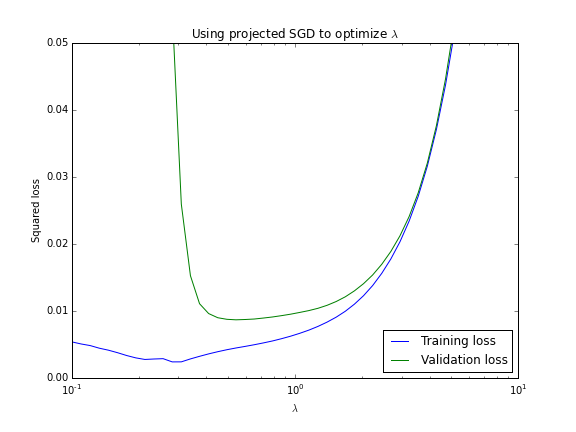
\includegraphics[scale=0.65]{./../figures/5_1.png} \end{center}

Note that projected SGD and coordinate descent find essentially the same solution. However, the validation set loss values obtained for projected SGD is much worse than those obtained for coordinate descent for $\lambda$ values that are not near $\lambda_{optimal}$.

\begin{center} 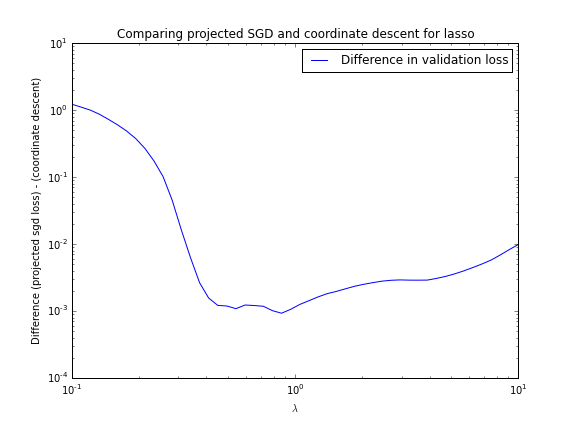
\includegraphics[scale=0.65]{./../figures/5_2.png} \end{center}

This behavior is likely due to lack of convergence (i.e. a function of the fixed stepsize in SGD, and the number of iterations for both algorithms).

\subsubsection*{5.2 Comparing projected SGD and coordinate descent}

Finally, the sparsity of the SGD solution is analyzed (using several thresholds for $w_j$ near zero):

\begin{itemize}

\item $w_j  = 0$:

\begin{center}
\begin{tabular}{| c | c | c |}
\hline
	& Predicted zero &  Predicted non-zero\\
\hline
True non-zero ($\bm{w}$[0:10]) &  0 &  10 \\
\hline
True zero ($\bm{w}$[10:]) & 0 & 65 \\
\hline
\end{tabular}\end{center}

\item $w_j < 10^{-3}$:

\begin{center}
\begin{tabular}{| c | c | c |}
\hline
	& Predicted zero &  Predicted non-zero\\
\hline
True non-zero ($\bm{w}$[0:10]) &  0 &  10 \\
\hline
True zero ($\bm{w}$[10:]) & 14 & 51 \\
\hline
\end{tabular}\end{center}

\item $w_j < 10^{-2}$:

\begin{center}
\begin{tabular}{| c | c | c |}
\hline
	& Predicted zero &  Predicted non-zero\\
\hline
True non-zero ($\bm{w}$[0:10]) &  0 &  10 \\
\hline
True zero ($\bm{w}$[10:]) & 57 & 8 \\
\hline
\end{tabular}\end{center}

\end{itemize}

Comparing our results to coordinate descent, it appears the coordinate descent algorithm finds the optimal solution more quickly (both in terms of minimum squared validation error and maximum sparsity). However, it is important to note the projected SGD algorithm has not been optimized- specifically, it was only run with a fixed step size of $\alpha = 0.0001$, which was selected since it found the correct $\lambda$.

%----------------------------------------------------------------------------------------


\end{document}